\begin{center}
    \begin{figure}[H]
        \centering

        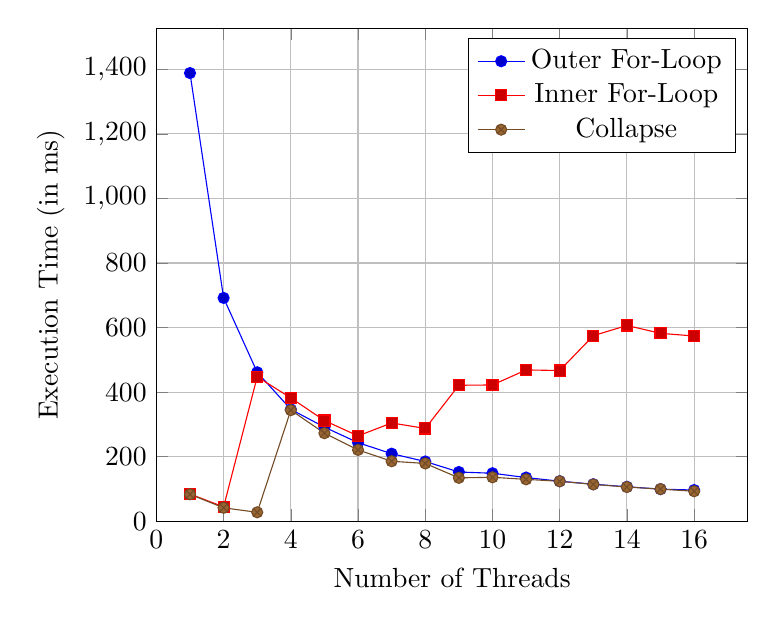
\begin{tikzpicture}
            \begin{axis}[
                title={},
                width=0.75\textwidth,
                xlabel={Number of Threads},
                ylabel={Execution Time (in ms)},
                xmin=0,
                ymin=0,
                grid=major
            ]
                \addplot coordinates {
                    (1,1388.14)(2,691.776)(3,461.453)(4,346.732)(5,291.6)(6,243.522)(7,209.415)(8,185.205)(9,152.677)(10,148.821)(11,135.525)(12,124.202)(13,114.814)(14,106.967)(15,99.6424)(16,96.8423)
                };
                \addlegendentry{Outer For-Loop}

                \addplot coordinates {
                    (1,84.6405)(2,44.5646)(3,447.501)(4,382.118)(5,311.966)(6,264.444)(7,304.552)(8,287.558)(9,421.305)(10,422.189)(11,468.759)(12,466.95)(13,574.857)(14,606.458)(15,582.076)(16,573.846)
                };
                \addlegendentry{Inner For-Loop}       

                \addplot coordinates {
                    (1,83.5909)(2,41.8099)(3,27.8556)(4,344.236)(5,272.88)(6,221.026)(7,185.961)(8,179.126)(9,134.584)(10,136.283)(11,129.925)(12,123.893)(13,114.326)(14,106.155)(15,99.6781)(16,93.0359)
                };
                \addlegendentry{Collapse}
            \end{axis}
        \end{tikzpicture}
        \caption{Grayscale Performance Tests dice\_large.png}
    \end{figure}
\end{center}